\section{Computational Model and System Overview}
In this section, we introduce the computational model for our
approach and give an overview of the Qsearch system and its components.

\subsection{Model for Facts, Queries and Answers}
\label{sec:framework}

%In this paper we present two models, the first is the \texttt{Quantity Fact Extraction} model and the second is the \texttt{Matching} model.
%We formalize the notions of quantity facts, quantity queries
%and answers to queries as follows. 

%In this section, we start by introducing some definitions to lay the foundation for our model. Then, we present our model and specify its inputs and outputs.

%In this section, we introduce our computational model for answering numerical queries, that would be exploited to develop our methodology to extract answers from text later on. In particular, we compose the following definitions:


%This numerical fact representation is quite close to the traditional RDF representation \cite{rdf},  which models each fact as a \textit{(subject, predicate, object)} triple. While the  entity $E$ and quantity $Q$ play as the \textit{subject} and \textit{object} in the RDF model respectively, the context $X$ works like a \textit{predicate}. However, instead of using a unique predicate for all the facts with the same predicate meaning as in the RDF model, we represent $X$ as a set consisting of tokens that could explain the connection between $E$ and $Q$. That is, in a sentence $S$ containing some entity $E$ and quantity $Q$, the context $X$ is determined as a subset of important words from $S$ which could clarify the role of $Q$ with regard to $E$. 


%%%%%%%%%%%%%%%%%%%%%%%%%%%%%%%%% QFE %%%%%%%%%%%%%%%%%%%%%%%
%\subsubsection{Quantity Fact Extraction Model}
\subsubsection{Extraction Model.}
%start from here 
The \textit{input} of this model is a corpus of text documents $\mathcal{T}$ with text snippets (e.g., sentences or paragraphs) that contain
%$n$ 
entity and 
%$m$ 
quantity mentions. 

The \textit{output} of this model is a set of \textit{quantity facts} extracted from the text corpus, $\mathbb{F} =\{\mathcal{F}_1, \mathcal{F}_2, ...\}$, where a quantity fact is defined as follows.


\begin{definition}[Quantity fact] A quantity fact (Qfact) is a triple $\mathcal{F} = (e,q,X)$, where: \\
- $e$ is an entity;\\
- $q = (v,u,r)$ is a quantity consisting of a numerical value $v$, a canonicalized unit $u$ (e.g., km, \$) and a value resolution $r$ (exact, approximate, upper/lower bound, %range
interval);\\
- $X = \{x_1,x_2,...\}$ is a context, which is a bag of words describing the relation between $e$ and $q$.
\end{definition}


\begin{example}
Given the text snippet \textit{``BMW i8 costs about 138k Euros in Germany and has a battery range between 50 and 60 km.''}, we can extract the following Qfacts:\\
- $\mathcal{F}_1: e=\textit{BMW i8}; q=\textit{(138.000, \euro, approximate)}; X = \{\textit{costs, Germany}\}$\\
- $\mathcal{F}_2: e=\textit{BMW i8}; q=\textit{(50-60, km, interval)}; X = \{\textit{range, battery}\}$ 
\qed 
\end{example}


The Qfact representation is similar to the RDF model
\cite{rdf}, 
which
represents each fact as a \textit{(subject, predicate, object)} triple.  In  the Qfact model,  the  entity $e$ and the quantity $q$  correspond to the \textit{subject} and the \textit{object}, respectively. 
The context $X$ in Qfacts is a proxy for the \textit{predicate} in the RDF model. However, it differs in two essential points: first, the context $X$ can capture more than one relation between $e$ and $q$; second, the context $X$ consists of a set of non-canonicalized tokens, instead of a unique canonicalized predicate in a knowledge graph. 

This relaxed representation is a judicious design choice and
essential for the flexibility of our approach: first, we can represent complex n-ary facts using a simple Qfact triple; second, our model can generalize to unseen relations; third, our model can cope with the 
inevitable diversity
and uncertainty in the language expressions of the underlying
text snippets. 
In theory, it is conceivable that all arguments that appear in
the context $X$ are also individually extracted and canonicalized
 to fill the slots of a frame-like structured record.
However, approaches along these lines do not work robustly and
suffer from heavy propagation of noise and errors.


The Qfact model allows different representations of the same fact,
and the underlying text corpus may express the same 
knowledge by different paraphrases. Hence, 
Qfacts are more expressive towards answering queries
via approximate matches and related phrases.
%provides a flexible model to represent the various information expressed in the text.

%%%%%%%%%%%%%%%%%%%%%%%%%%%%%%%%%%%%%%%%%%%%%%%%%%%%%%

%%%%%%%%%%%%%%%%%%%%%%Matching
\subsubsection{Matching Model.}

The \textit{input} of this model is a set of Qfacts $\mathbb{F} =\{\mathcal{F}_1, \mathcal{F}_2, ...\}$
extracted from the text corpus, and  a \textit{quantity query} $\mathcal{Y}$ defined as:


\begin{definition}[Quantity query] A quantity query (Qquery) is a triple $\mathcal{Y} = (t^*,q^*,X^*)$ where: \\
- $t^*$ is the semantic type of the target answers;\\
- $q^* = (v,u,o)$ is a quantity condition consisting of a numerical value $v$, a canonicalized unit $u$ 
(e.g., km, \$)
, and a comparison operator $o$ (exact, approximate, upper/lower bound, 
%range
interval);\\
- $X^* = \{x_1,x_2,...\}$ is a context condition, 
expressed by a bag of words that describes the 
relation between $t^*$ and $q^*$.
\end{definition}

\begin{example}
\label{ex:qquery}
Given the query \textit{``Cars with price less than 100k Euros in Germany''}, its corresponding Qquery is  as follows:\\
- $\mathcal{Y} : t^* = \textit{car}; q^*=\textit{(100.000, \euro, upper bound)}; X^* = \{\textit{price, Germany}\}  $
\qed 
\end{example}

%The definition of the Qquery is analogous to that of the Qfact. Such that, 
Each part of a Qquery imposes a constraint on its 
counterpart in a Qfact considered as a candidate answer.

\begin{definition}[Query answer] 
 A Qfact $ \mathcal{F} =(e,q,X)$ is an answer for a Qquery $\mathcal{Y} = (t^*,q^*,X^*)$ iff 
(1) $e$ is an entity of type $t^*$, 
(2) the quantity $q$ satisfies the quantity condition $q^*$ and (3) the context $X$ (approximately) matches the context condition $X^*$.
\end{definition}

\begin{example}
Consider the Qquery in Example \ref{ex:qquery} and the two text segments
 \textit{``German dealers sell the BMW X3
 at a price as low as 55,000 Euros''} and
 \textit{``Car dealers in Munich sell the BMW X3
starting at 55,000 Euros''}.
The Qfact extracted from the first snippet
with 
$e=\textit{BMW X3},
q=\textit{(55.000, \euro, lower bound)}$,
and $X = \{\textit{German, dealers, sell, price}\}$
is a strong match for the query;
whereas the Qfact extracted from the second snippet
with 
$e = \textit{BMW X3},
q=\textit{(55.000, \euro, lower bound)}$,
and $X = \{\textit{car, dealers, Munich, sell}\}$
is an approximate match (by embedding-based relatedness).
\qed 
\end{example}

The \textit{output} of this model is a ranked list of entities $\mathcal{E}^* = \{e_1, e_2, e_3,...\}$ from matching Qfacts with the Qquery, which will be discussed in Section \ref{sec:match}.

%%%%%%%%%%%%%%%%%%%%%%%%

\subsection{Qsearch System}
Figure \ref{fig:system} 
%shows the high-level architecture of 
gives an overview of the architecture of 
Qsearch. The arrows in the figure depict information flow between the different system components. 
Qsearch consists of two main stages:
\textit{Extract}
and \textit{Answer}.
 
%In this section, we demonstrate our numerical question answering system from text. In Figure \ref{fig:system}, we present a high-level architecture of our system, where the arrows depict information flow between building blocks. We split the working flow of our system into two main stages: \textit{Extract} and \textit{Answer}.

\begin{figure}[t]
\centering
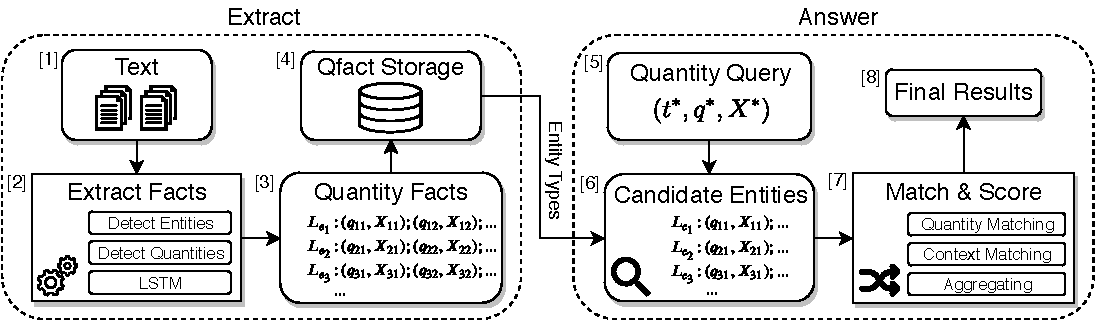
\includegraphics[width=1\textwidth]{figures/overview.pdf}
\caption{Overview of Qsearch.}
\label{fig:system}
\end{figure}
% what is the storage, how is it stored, and indexed 

\subsubsection{Extract.}  
We preprocess the text corpus (Block 1) to recognize
and disambiguate named entities 
%using the AIDA \cite{DBLP:conf/emnlp/HoffartYBFPSTTW11} system,
%which links named entities to the YAGO knowledge base\cite{DBLP:conf/www/SuchanekKW07}. 
and link them to an external knowledge base (KB). We also identify mentions of quantities in the text and normalize them into standard units. 
Subsequently, we run a deep neural network to extract Qfacts from the preprocessed text (Block 2). We learn and employ a specifically designed
Long Short Term Memory (LSTM) network, which will be described in Section \ref{sec:extract}. 

Extracted Qfacts are organized and grouped by their named entities, such that each individual entity $e_i$ is mapped to a list of quantities and related contexts $L_{e_i} = \{(q_{i1},X_{i1}),(q_{i2},X_{i2}),... \}$ (Block 3).
All extracted Qfacts are stored in a data repository (Block 4, 
based on Elasticsearch in our implementation), where entities are linked to their semantic types from the KB.
%We use AIDA \cite{DBLP:conf/emnlp/HoffartYBFPSTTW11} for entity linking, YAGO \cite{DBLP:conf/www/SuchanekKW07} for entity typing, and ElasticSearch as a storage engine.



\subsubsection{Answer.}
We answer incoming Qqueries by matching them against
the Qfacts from the \textit{Extract} stage. 
For a Qquery $(t^*,q^*,X^*)$ (Block 5), we first apply 
an entity-type filter, eliminating entities with the wrong type. 
This results in a set of candidate entities $\mathcal{C} = \{c_1,c_2,...\}$ (Block 6) satisfying the type constraint $t^*$, along with their quantity-context pairs $\{L_{c_1},L_{c_2},...\}$. 
In Block 7, we discard all candidate answers 
%with quantity-context pairs $(q,X) \in L_c$ 
that do not satisfy the quantity condition $q^*$.
Finally, we compute a matching score for each candidate entity $c \in \mathcal{C}$ based on the contexts $X$ in the
quantity-context pairs $L_c$, using a statistical language model
or a text embedding method, which will be described in Section \ref{sec:match}. The candidate entities are ranked by their scores and returned to the user (Block 8). 

In the following Sections
\ref{sec:extract} and \ref{sec:match}, we discuss in detail the
 Qfact extraction model and the matching and answering model, 
respectively.

%In the remainder of this section, we discuss how each candidate entity is scored in Block 7.
